\section{Recolección}

%-------------------------------Recolección----------------------------------------------%

El proceso de recolección es parte fundamental del presente trabajo terminal, ya que permitió conformar el corpus necesario para llevar a cabo la etapa de entrenamiento, este proceso se llevo a cabo por etapas.

\begin{itemize}
	\item Seleccionar los sitios web
	\item Información a recolectar
	\item Análisis del sitio web
	\item Proceso de recolección
\end{itemize}

\subsection{Selección de sitios web}

Se han seleccionado los diarios Aristegui Noticias, El Economista, La Jornada, La Prensa, Proceso, Sopitas y TV Azteca para recolectar noticias, fueron seleccionados debido a que forman parte de los sitios web más consultados, sin embargo durante la etapa de recolección se descartaron ciertos sitios debido a que ya no permiten realizar \textit{web scraping}


\subsection{Información recolectada}

Se llevó a cabo un análisis acerca de la información que contiene cada una de las noticias y con base en ello se determinó recolectar la siguiente información:

\begin{itemize}
	\item URL de la noticia
	\item Título
	\item Fecha
	\item Sección
	\item Autor
	\item Descripción
	\item Noticia
\end{itemize}

Cabe destacar que no toda la información recuperada fue utilizada en el proceso de entrenamiento, sin embargo se considerarón los puntos anteriores ya que la mayor parte de las noticias cuentan con esa información.


\subsection{Análisis de sitios web}

Una vez definida la información requerida de cada noticia se realizó un análisis sobre la estructura HTML de cada sitio web, con el fin de realizar expresiones \textit{XPath} que nos permitieran recorrer y procesar un documento XML, dado que cada sitio web cuenta con una estructura diferente, fue necesario realizar el análisis de manera individual, cabe mencionar que existen sitios los cuales realizan actualizaciones a sus páginas por lo cual era necesario realizar el análisis cada dos meses.

Una expresión \textit{XPath} de ruta nos permite buscar y seleccionar los distintos nodos de un documento XML, en el siguiente Cuadro \ref{box:xmlEjemplo} se muestra un ejemplo de un documento XML.

\begin{mygraybox}[label={box:xmlEjemplo}]{Documento XML} 
<nota>\\
	<para>Daniel</para>\\
	<de>Andres</de>\\
	<titulo>Recordatorio</titulo>\\
	<texto>Don't forget me this weekend!</texto>\\
</nota>
\end{mygraybox}

\subsection{Proceso de recolección de noticias}

Existen diversas técnicas y herramientas para la recolección de información, sin embargo en el presente trabajo han sido utilizadas técnicas de \textit{web scraping}.

La siguiente Figura \ref{Fig:recoleccion} muestra el proceso que se lleva a cabo durante la recolección utilizando web scraping.

\begin{figure}[H]
	\centering
	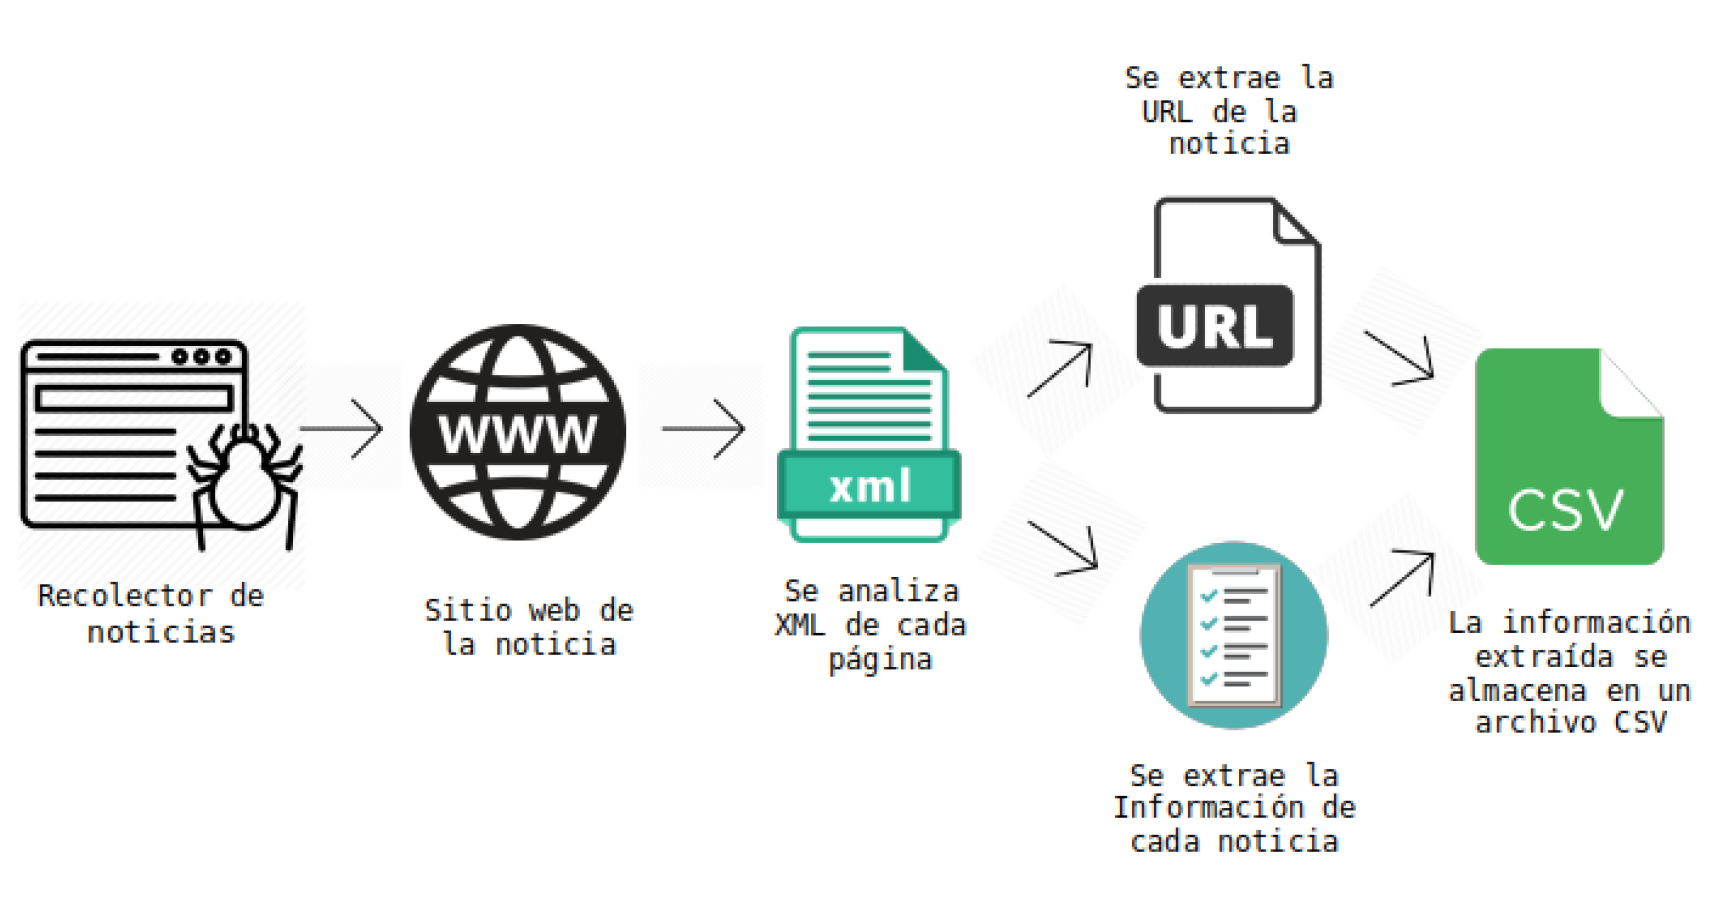
\includegraphics[scale=.2]{imagenes/Capitulo5/recoleccion.png}
	\caption{Proceso de recolección}
	\label{Fig:recoleccion}
\end{figure}

Es necesario contar con noticias de las secciones (Ciencia y Tecnología, Cultura, Deportes, Economía y Política), por lo cual se realizó un crawler por sección, con el fin enriquecer el número de noticias de cada sección, permitiendo obtener mejores resultados en la práctica.
\\
Para generar nuestro corpus, se recolectaron noticias durante el periodo de julio a septiembre con un intervalo de dos días, con el fin de no tener noticias repetidas y evitar ser bloqueados debido alnúmero de peticiones realizadas al sitio web. 
\\
Una vez finalizado el proceso de recolección los resultados obtenidos por sección se muestra en la Figura  \ref{Fig:notseccionV1}.

\begin{figure}[H]
	\centering
	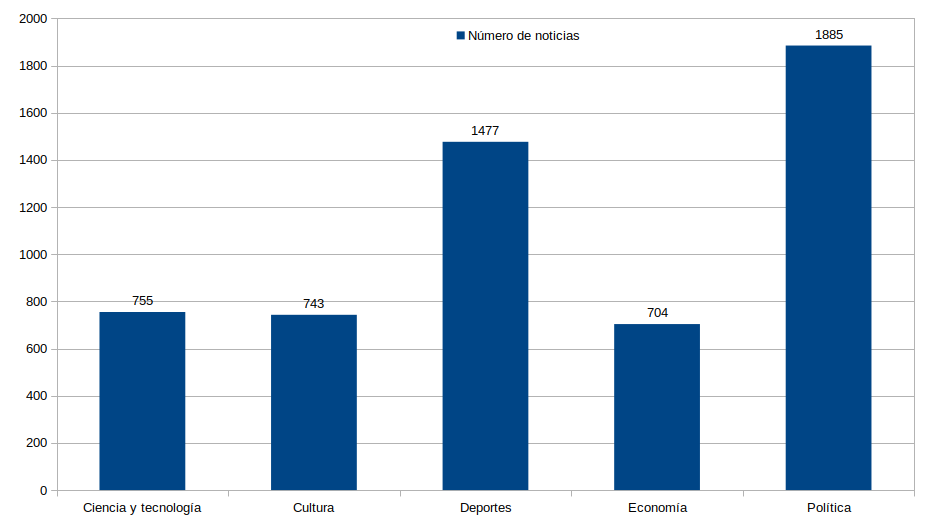
\includegraphics[scale=.6]{imagenes/Capitulo5/noticiasPorSeccionV1.png}
	\caption{Noticias recolectadas durante el primer corte.}
	\label{Fig:notseccionV1}
\end{figure}

Cabe destacar que el número de noticias por sección no se encontraba balanceado debido a que no existía un gran número de sitios que publicarán noticias de cultura, por ello se decidió continuar con el proceso de recolección de noticias, con el fin de balancear el corpus y así nuestros resultados obtenidos en la práctica fueran mejores.
\\
Una vez finalizada la segunda etapa de recolección los nuevos resultados se muestran en la Figura \ref{Fig:notseccion}

\begin{figure}[H]
	\centering
	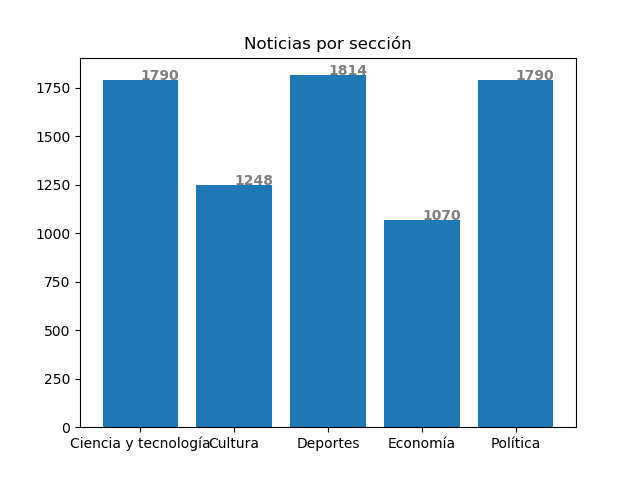
\includegraphics[scale=.6]{imagenes/Capitulo5/noticiasPorSeccion.png}
	\caption{Numero total de noticias recolectadas por sección.}
	\label{Fig:notseccion}
\end{figure}

Las resultados obtenidos por cada sitio web, se muestran en las siguientes Figuras.
\\
\begin{figure}[H]
	\centering
	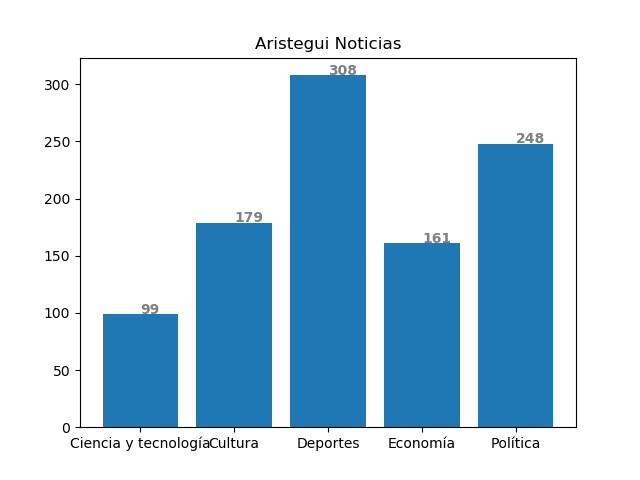
\includegraphics[scale=.45]{imagenes/Capitulo5/aristegui.png}
	\caption{Total de noticias recolectadas del sitio web de Aristegui Noticias}
	\label{Fig:notsitioaristegui}
\end{figure}

\begin{figure}[H]
	\centering
	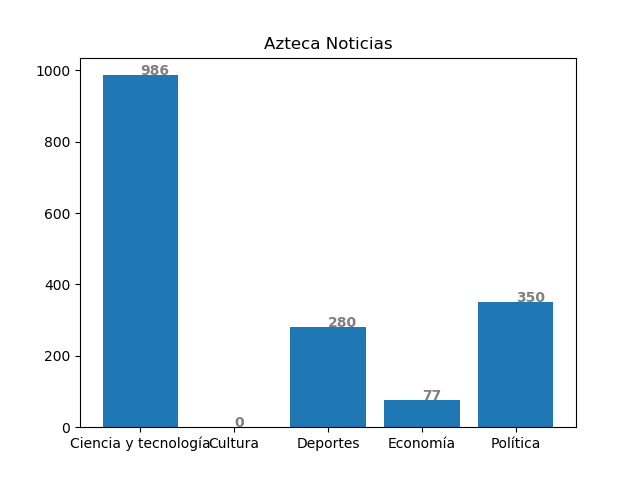
\includegraphics[scale=.45]{imagenes/Capitulo5/azteca.png}
	\caption{Total de noticias recolectadas del sitio web de Azteca Noticias}
	\label{Fig:notsitioazteca}
\end{figure}

\begin{figure}[H]
	\centering
	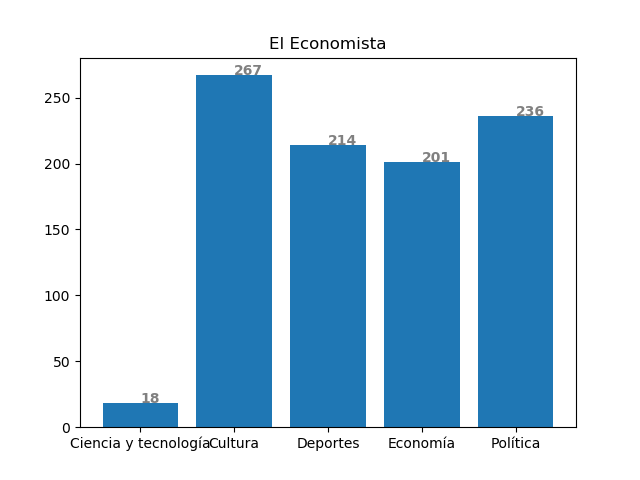
\includegraphics[scale=.45]{imagenes/Capitulo5/economista.png}
	\caption{Total de noticias recolectadas del sitio web de El Economista}
	\label{Fig:notsitioeconomista}
\end{figure}

\begin{figure}[H]
	\centering
	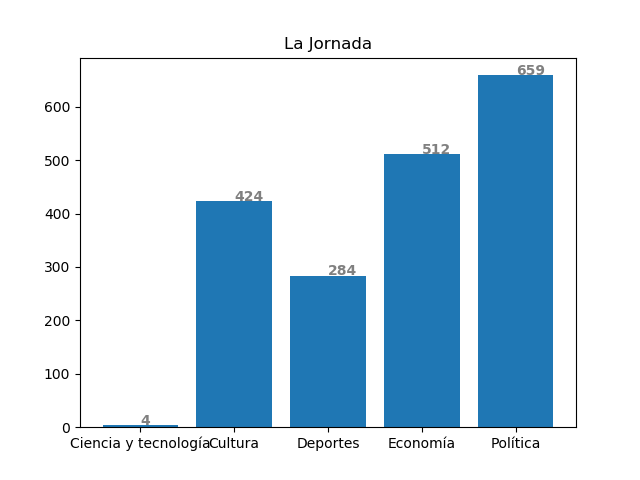
\includegraphics[scale=.45]{imagenes/Capitulo5/jornada.png}
	\caption{Total de noticias recolectadas del sitio web de La Jornada}
	\label{Fig:notsitiojornada}
\end{figure}

\begin{figure}[H]
	\centering
	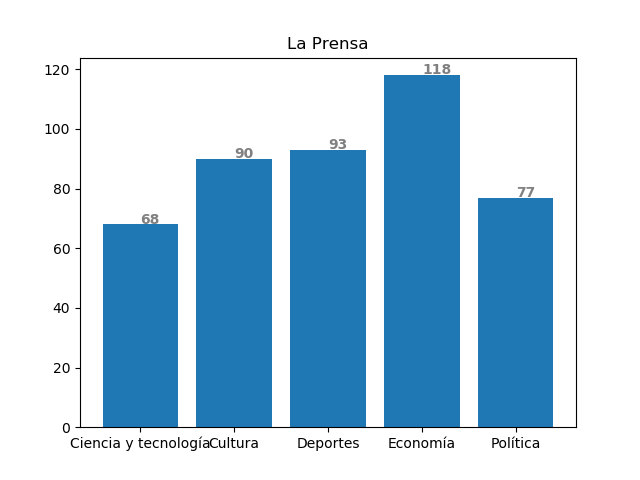
\includegraphics[scale=.45]{imagenes/Capitulo5/prensa.png}
	\caption{Total de noticias recolectadas del sitio web de La Prensa}
	\label{Fig:notsitioprensa}
\end{figure}

\begin{figure}[H]
	\centering
	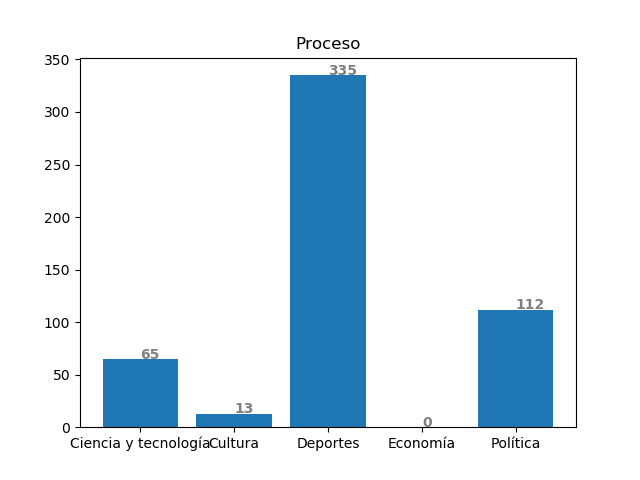
\includegraphics[scale=.45]{imagenes/Capitulo5/proceso.png}
	\caption{Total de noticias recolectadas del sitio web de Proceso}
	\label{Fig:notsitioproceso}
\end{figure}

\begin{figure}[H]
	\centering
	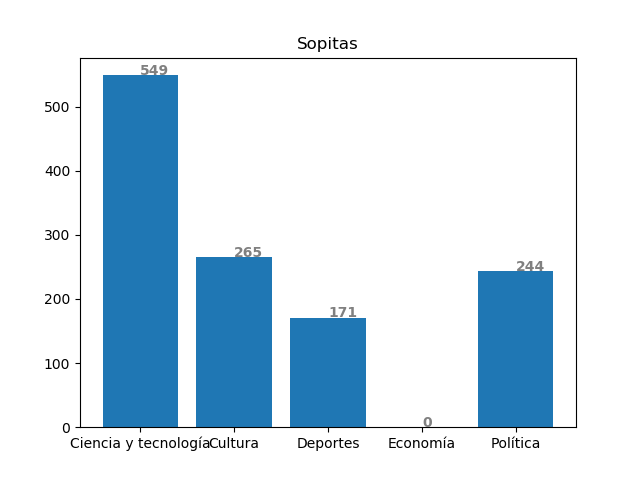
\includegraphics[scale=.45]{imagenes/Capitulo5/sopitas.png}
	\caption{Total de noticias recolectadas del sitio web de Sopitas}
	\label{Fig:notsitiosopitas}
\end{figure}

Una vez concluida la recolección de noticias se procedió con el balanceo de noticias quedando un total de 700 noticias por sección.